\documentclass[letterpaper,11pt]{article}
\usepackage[margin=1in]{geometry}
\usepackage{graphicx}
\graphicspath{ {./images/} }
\begin{document}

\section{Introduction}
%Lay out "the vision"
New blockchain technologies are the subject of much hype and speculation. Some of these technologies may have DoD applications, but assessing what they are capable of and under what circumstances is an ongoing challenge to researchers. Building upon past work that investigated and taxonomized the true capabilities of various blockchain technologies, we present here the next step in such analysis and understanding. We have designed and built a simulation platform for comparing blockchain technologies against one another and investigating their properties under a variety of circumstances. We hope that this platform will allow researchers to further scrutinize and assess blockchain technologies for their suitability for different purposes.

\section{Simulation Design}
The simulation program has two major components: a graph of Miner objects that will participate in a blockchain protocol, and an abstraction of the transactions they will create and attempt to come to consensus on. Other modules, including simulation settings and a system for determining what transaction should be generated next, support these two main components. Note that although it may not be accurate to call the entities that handle transactions in a given blockchain protocol ``miners'', we do so here for simplicity.

\subsection{Graph of Miners}
The simulated miners are arranged in a undirected graph whose topology is specified by the simulation settings. The topology can be loaded from a file or generated randomly. Each node in the graph stores a Miner object that will participate in the protocol. The miners' views of the blockchain start with all miners in consensus about a genesis transaction.

At every time step of the simulation, each miner receives and processes messages, updates the consensus states of the transactions in its view of the blockchain (i.e. whether they are in consensus or not), and attempts to generate a new transaction. Furthermore, each miner is given the opportunity to indicate that some of its transactions should be reissued. The details of how miners carry out these actions is protocol-dependent and will be discussed in the appropriate subsections below.

Messages are passed along edges in the graph to simulate a P2P network. Each miner receives messages from other miners and broadcasts any transactions that it sees for the first time (whether because it is newly created or the first time a neighbor has sent the transaction). The simulation can assign a message delay in the form of a probability distribution to any edge. When messages are sent along that edge, the distribution is sampled and the message is delayed for the appropriate number of time steps. In its current implementation, the simulation does not support message loss.

The real-world time represented by the simulation's time steps is based on the message delay. For example if message delay in the simulation is modeled by a negative exponential distribution between approximately 1--10 time steps, and messages are delayed anywhere between 50--500ms on the Internet [citation needed], then each time step represents approximately 50ms of real-world time.

\subsection{Transactions}
Blockchain transactions in the real world contain specific information and correspond to state changes that must be verified against the other transactions in the ledger. For the purposes of this simulation, however, the contents of the transactions are irrelevant. Thus, each transaction has an identifier that takes the place of any state change information that would be contained in a real-world transaction. We are only concerned with how the miners come to consensus about transactions, not the state changes they represent. 

For similar reasons, we have also abstracted away the concept of ``blocks'' entirely. A real-world block is a set of transactions with a pointer (or multiple pointers, as is the case for Iota) to a previous block in the form of that block's hash. If a block were to contain only one transaction, it would be functionally identical to a transaction that stores its own hash pointer(s). In this simulation, Transaction objects are precisely that. They contain simply an identifier, any number of hash pointers, and some metadata that is useful for reporting on the outcome of the simulation.

\subsection{Transaction Generation}
At every step of the simulation, each miner has a chance to create a new transaction (block). The identifier assigned to the newly generated transaction is either never-before-seen or a reissue of a previous transaction that was not accepted into the blockchain. This allows a transaction that the miners did not reach consensus for to get another chance to be included in the blockchain, which mirrors how originators of transactions in the real world will submit them for inclusion into blocks until they are accepted.

The rate at which new transactions are generated is a configurable setting of the simulation. Settings provide a target number of time steps that should pass on average between transaction generation. Furthermore, each miner has an integer mining power value associated with it that indicates its relative chance to be selected as the miner to create a new transaction. With these two parameters, the simulation has a random chance of generating a new transaction every time step such that on average the target number of time steps will pass between generations. If the random chance comes up in favor of creating a new transaction, a miner is chosen at random, weighted by mining power, to be the one to create the transaction. Of course, this differs from the mechanics by which any individual miner participating in a real-world blockchain protocol would generate a new transaction. However, this method is an acceptable abstraction because it still reaches the target generation rate and is more computationally efficient.

\subsection{Protocols}
The purpose of this simulation is to compare the properties of various blockchain protocols. As such, the system can be configured to run with different protocols. The two that are currently implemented are Bitcoin and Iota. Both of these protocols are simulated using the same framework of Miner objects in a graph that exchange transaction messages with one another. What differs between them is what consensus protocol the miners execute.

The simulation is designed to be extensible to allow for other protocols to be simulated. By inheriting from the Miner class or any existing protocol, a new protocol class can be simulated with the same time step and P2P messaging model.

Our simulations of both the Bitcoin and Iota protocols function similarly. Both protocols maintain directed acyclic graphs (DAGs) of their respective blockchain views. Nodes in Bitcoin miners' DAGs have exactly one hash pointer, and nodes in Iota miners' have exactly two (excluding the genesis transaction and the first non-genesis transaction in Iota).

When a Bitcoin or Iota miner receives a message and learns of a transaction for the first time, it uses the transaction's hash pointer(s) to position it in the miner's view. The transactions that correspond to a transaction's hash pointers are that transaction's ``parents''. If the miner receives a new transaction but doesn't have all of its parent in its view, it stores the new transaction as an ``orphan'' and requests the missing transaction(s) from the miner who sent the message. Every time the miner learns of a new transaction it goes through all of its orphans and looks for their hash pointers in its view, adding an orphan to the view when its parents are found.

Where the Bitcoin and Iota protocols differ is in how parents are chosen for newly created transactions and how miners running those protocols update their states about each transaction in their view.

When a Bitcoin miner creates a new transaction, it chooses as its parent the deepest transaction in its view of the blockchain, chosen randomly in the case that there are more than one at that depth. An Iota miner that creates a new transaction will choose as its parents two transactions that have no transactions pointing to them, called ``frontier transactions'' or ``tips''. If there are more than two frontier transactions, two are selected at random. In the case where there is only one frontier transaction, another transaction in the DAG is selected at random as the second parent.

Bitcoin miners consider a transaction to be in consensus when it is on the longest fork of the chain and is a certain height above the deepest node in the chain. Canonically this height is six, but that is a configurable setting in the simulation. Bitcoin miners track the transactions they have created and reissue them if they end up on a fork of the blockchain. A tracked transaction is only reissued after consensus is reached for the transaction on the main chain with equivalent depth to the tracked transaction.

Iota miners consider a transaction to be in consensus when it is reachable by all frontier transactions by recursively following the hash pointers of each frontier transaction. Iota miners do not reiusse transactions, because it is unclear when a transaction can be considered with some confidence to never be able to be in consensus.

\subsection{Monte Carlo Simulation}
Blockchain consensus protocols proceed with a significant amount of randomness. Transactions are generated and added to the blockchain with an element of randomness which can cause similar simulation setups to yield very different results. As such, the simulation employs the Monte Carlo method of running a high number of simulations with the same parameters to get better data about overall trends. When data from multiple runs of the simulation are combined, they tell a clearer story about the behavior of the protocol and smooth out any outlying data that resulted from the random processes involved in the protocol.

Multithreading allows multiple runs of the simulation to proceed in parallel. The simulation starts up a configurable number of workers that each run simulations until the total number of runs reaches a specified value.

\subsection{Simulation Settings}
The simulation includes protocol, graph topology, and simulation settings that can be used to simulate different protocols under various conditions. Bitcoin or Iota can be specified as the protocol to simulate, along with parameters for the target number of time steps that should pass on average between transaction generation. The Bitcoin protocol settings also include the depth at which a Bitcoin miner will consider a transaction accepted if it is on the longest chain.

The settings for network graph topology include the option to use a static or randomly generated graph (including generation parameters), the number of miners to be simulated, and the probability distribution from which edge delays should be sampled.

The general simulation settings control how many runs should be executed in the Monte Carlo simulation, how many workers should participate in multithreading, and when each simulation should terminate. Every simulation reported here ran until a certain number of transactions were created, then allowed the miners to finish exchanging messages before terminating. Settings also control the distribution of miner power by allowing a probability distribution of miner power to be specified as well as a list of mining power percentages for the top miners. This last parameter is helpful for modeling a realistic network of Bitcoin miners where power distribution is heavily weighted toward a few miners.

\subsection{Simulation Data and Analysis}
The two metrics that we are primarily interested in for any given consensus protocol are the time it takes for miners to come to consensus on each transaction and the number of transactions that are in consensus at one point of the simulation and then move out of it. These metrics reflect critical properties for a blockchain currency because they dictate when the parties participating in a transaction can act on the currency exchange (e.g. by exchanging goods). The property of whether and how often transactions move out of consensus is especially critical because once a transaction is made it must be final.

The primary metadata that the simulation maintains for each transaction is a history of when each miner's state changed for that transaction. This history allows us to calculate consensus time for each transaction and record the instances when it moved out of consensus. The simulation reports these values as a CDF and a number, respectively.

\subsection{Limitations and Challenges}
Any abstract model of a real-world system incorporates simplifications that cause the model to deviate from reality. This section outlines the major limitations of our abstraction and provides justifications for the decisions we made.

\subsubsection{Transaction Creation and Validation}
As our model abstracts away realistic state changes from transactions, we make the assumption that whenever a miner is ready to create a new transaction that there is a state change that needs to be represented by it. As long as the rate of state changes is faster than the rate of transaction generation, then this model still reflects reality. If it became necessary to model this more granularly, then the component that issues identifier could be modified to accrue identifiers, representing state changes, over time and decline issuing an identifier if its pool of state changes is empty.

Validating that transactions represent valid state changes given the transaction history is an important task in real-world blockchain protocols. However, as our model abstracts away such changes from Transaction objects, we do not simulate transaction validation. All transactions generated by the simulation are assumed to be valid, and adding invalid transactions to the simulation is left as future work. 

Some concept of valid and invalid transactions could be added to the simulation without significantly shifting the level of abstraction employed by the model. For example, in addition to an identifier, a Transaction object could also be flagged as ``invalid'' or include a list of other transactions that it conflicts with (and should therefore never be included in the transaction history with). Either of these options could be useful for simulating malicious miners that propagate invalid transactions and the effect they have on consensus protocols.

\subsubsection{Network Topology and Properties}
Due to the collaborative nature of consensus protocols, the topology of the miner network impacts the results of the protocol. In order to collect correct data, we need to simulate the protocols as realistically as possible. Unfortunately, Bitcoin's topology is still partially unknown. Iota's topology is also unknown, and the current rate of transaction generation does not satisfy the conditions necessary for the protocol to run without a centralized coordinator. As such, we have estimated realistic properties for Bitcoin and Iota networks. We will examine the particulars of the simulations settings we use for each protocol in the following section, but we do note here that we use a random geometric graph in order to achieve a topology wherein nodes have varying levels of connectedness.

Communicating over the real-world Internet involves risks of delays and dropped messages. The simulation incorporates message delay into the communication between miners in order to simulate how this would affect consensus protocols, but it doesn't model messages being dropped. As these network-level considerations are not directly governed by the consensus protocol, we can simply assume that the simulated protocol operates on top of a communication layer that handles resending dropped messages.

\subsubsection{Iota Specification}
Iota's DAG-based approach to blockchain technology is particularly interesting to us, but while researching it we had difficulty finding clear and consistent sources on how it operates.

\section{Results}
In this section we describe the experiments we ran with the simulation platform and their results.

\subsection{Realistic Bitcoin}
The first experiment we ran was a simulation of Bitcoin with realistic parameters. This served as both a test of the system against the best understood blockchain protocol and as somewhat of a stress test, 

\subsubsection{Parameters}
We ran this simulation of Bitcoin with 2000 miners arranged in a random geometric graph with connectivity threshold 0.125. This number is lower than the estimated number of nodes that participate in the real-world Bitcoin protocol. However, the difference between 2000 and 4000 Bitcoin miners is negligible due to how power is distributed among real-world Bitcoin miners. The distribution of power among Bitcoin miners is such that over 95\% of mining power rests with the top 21 miners. Our simulation settings mirror this reality by setting the mining power of the top 21 miners so that it is  equal in proportion to that of the respective power of the top real-world miners. This results in all of the non-top-21 miners having less than a 0.002\% chance to generate a transaction when a miner is chosen to do so, compared to the top 3 miners' chances of 22.05\%, 13.95\%, and 11.8\%, respectively.

This simulation had a target transaction generation rate of once every 6000 time steps, with an exponential message delay of between 1 and 10 steps. Assuming that Internet message delay is between 100 and 1000ms, one time step is approximately equivalent to 100ms, giving a simulated target transaction generation rate of once every 10 minutes. This matches the generation rate of real-world Bitcoin.

The simulation ran until it had generated 30 transactions.

\subsubsection{Results}
%mention # of MC runs here (bc it's not really a param)
Forthcoming.

\subsection{Current-day Iota}
Similar to the realistic Bitcoin simulation described above, we ran an experiment to simulate how Iota runs today.

\subsubsection{Parameters}
We have estimated Iota's topology and protocol parameters based on the information that we could gather about the protocol. Estimates for the number of Iota nodes operating today range from 500--1000, and Iota monitors report a current rate of about 10 new transactions per second.

We ran this simulation with 500 Iota miners, all of equal power, arranged in a random geometric graph with connectivity threshold 0.125. An exponential message delay of between 10 and 100 steps, given an Internet message delay of 100--1000ms, means that time steps are approximately equivalent to 10ms. We set a target transaction generation rate of once every 10 time steps, which gives a rate of 10 transactions per second.

\subsubsection{Results}
Forthcoming.

\subsection{Sparse vs. Dense Bitcoin}
The network topology of the miners participating in a blockchain consensus protocol 

\subsubsection{Parameters}

\subsubsection{Results}

\subsection{NAME}

\subsubsection{Parameters}

\subsubsection{Results}

\subsection{Other Insights}
%"What I learned"

Investigating blockchain consensus protocols via direct simulation has yielded several interesting insights.

The distribution of power among Bitcoin miners is an important consideration for the protocol. The more power an entity controls, the more they can tamper with or disrupt the blockchain. When mining power is distributed as unevenly as it is in the current Bitcoin landscape, however, the resulting blockchain has fewer forks because the same few miners are the ones adding to the chain, increasing the likelihood that their personal views of the blockchain are up-to-date.

One of the major questions facing Iota is when to consider a transaction in consensus.

Waiting (20--30) time steps to check Iota consensus reduces instability.

What else?

\subsection{Future Work}
Malicious miners

Dynamic graphs

Other protocols, including newly invented ones

\subsection{Assorted Results}
These sections serve to preserve interesting results gathered from experimenting with the protocols in the simulation. These results are not meant to be published as-is and should be rewritten and incorporated into the main text, above.

\subsubsection{Realistic Bitcoin}
\begin{verbatim}
{
    "threadWorkers": 8,
    "numberOfExecutions": 1144,
    "topologySelection": "GENERATE_ONCE", 
    "terminationCondition": "NUMBER_OF_GENERATED_TRANSACTIONS",
    "topMinerPower": [22.05, 13.95, 11.8, 11.51, 9.17, 9.07, 3.61, 1.85, 1.76, 1.66, 1.56, 1.37, 1.37, 1.27, 0.98, 0.88, 0.78, 0.59, 0.59, 0.39, 0.29],
    "terminationValue": 30,
    "minerPower": {
        "type": "CONSTANT",
        "value": 1
    },

    "topology": {
        "type": "GEOMETRIC_UNIFORM_DELAY",
        "radius": 0.05,
        "numberOfMiners": 2000,
        "networkDelay": {
            "type": "EXPONENTIAL",
            "beta": 0.5
        }
    },
    "protocol": {
        "type": "BITCOIN",
        "acceptDepth ": 6,
        "targetTicksBetweenGeneration": 6000
    }
}
\end{verbatim}

These parameters reflect a realistic estimate of the real-world Bitcoin mining network. 2000 miners is smaller than the estimated number of miners (4000--7000) but is a reasonable abstraction because not all real-world miners mine blocks and they may collaborate in pools that can be thought of as one ``effective miner''.  Percent power share of the top 21 miners was drawn from \verb|https://btc.com/stats/pool?pool_mode=week| on July 11, 2018. The exponential distribution for message delay with a beta of 0.5 is rounded to only give integer results. This results in message delays exponentially distributed between 1 and 10 time steps. That, combined with a target transaction generation rate of one transaction every 6000 ticks, and given that real-world Internet delay is exponential between 100ms and 1000ms means that one time step is approximately 10ms.

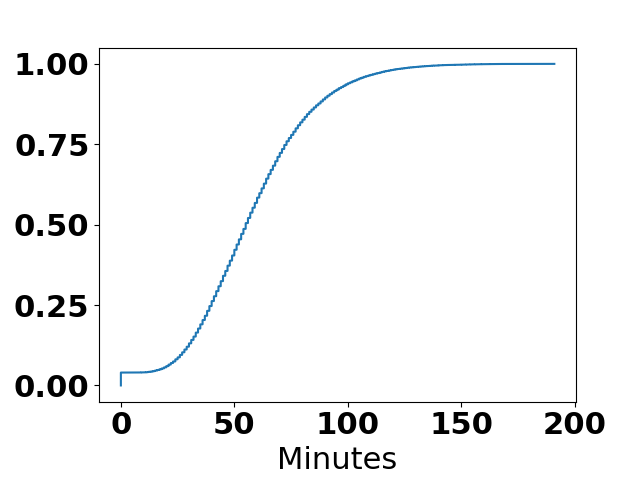
\includegraphics[scale=0.5]{realbctimes}

The results of running the simulation with these parameters give a consensus time of <60 minutes on average. This is a bit on the high side, but is a reasonable result when compared to the ground truth of how Bitcoin operates today.

These results eclipse various runs with less realistic density (see below) or fewer Monte Carlo runs. That data is therefore not included.

\subsubsection{Denser Bitcoin}
This run of the simulation is similar to the above, but only contains 264 runs. It was run with a less realistic topology: much more dense than is realistic (geometric with radius 0.0125). Note that the \textit{combination} of number of miners and geometric radius determine the density of the topology (so with a fixed radius, the graph will be sparser with fewer miners and denser with more miners).

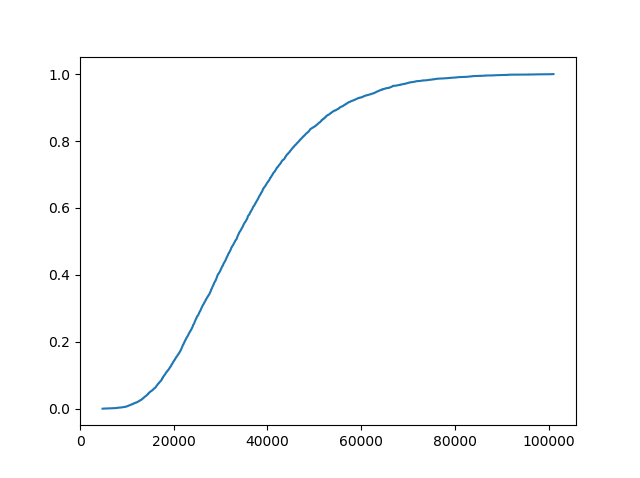
\includegraphics[scale=0.5]{densebctimes}

As expected, the average consensus time is reduced. One time step here is approx. 10ms, so average is close to 30 minutes.

\subsubsection{Comparing Bitcoin}

We compared Bitcoin's performance when running on a sparse (linear) vs. realistically dense (geometric with radius 0.05) topology. We also compare different transaction generation rates (6s, 60s, 600s) and realistic (same as above) and high latency (I think the networkDelay ``beta'' was 100, but I don't have the data). These simulations were run with uniform miner power.

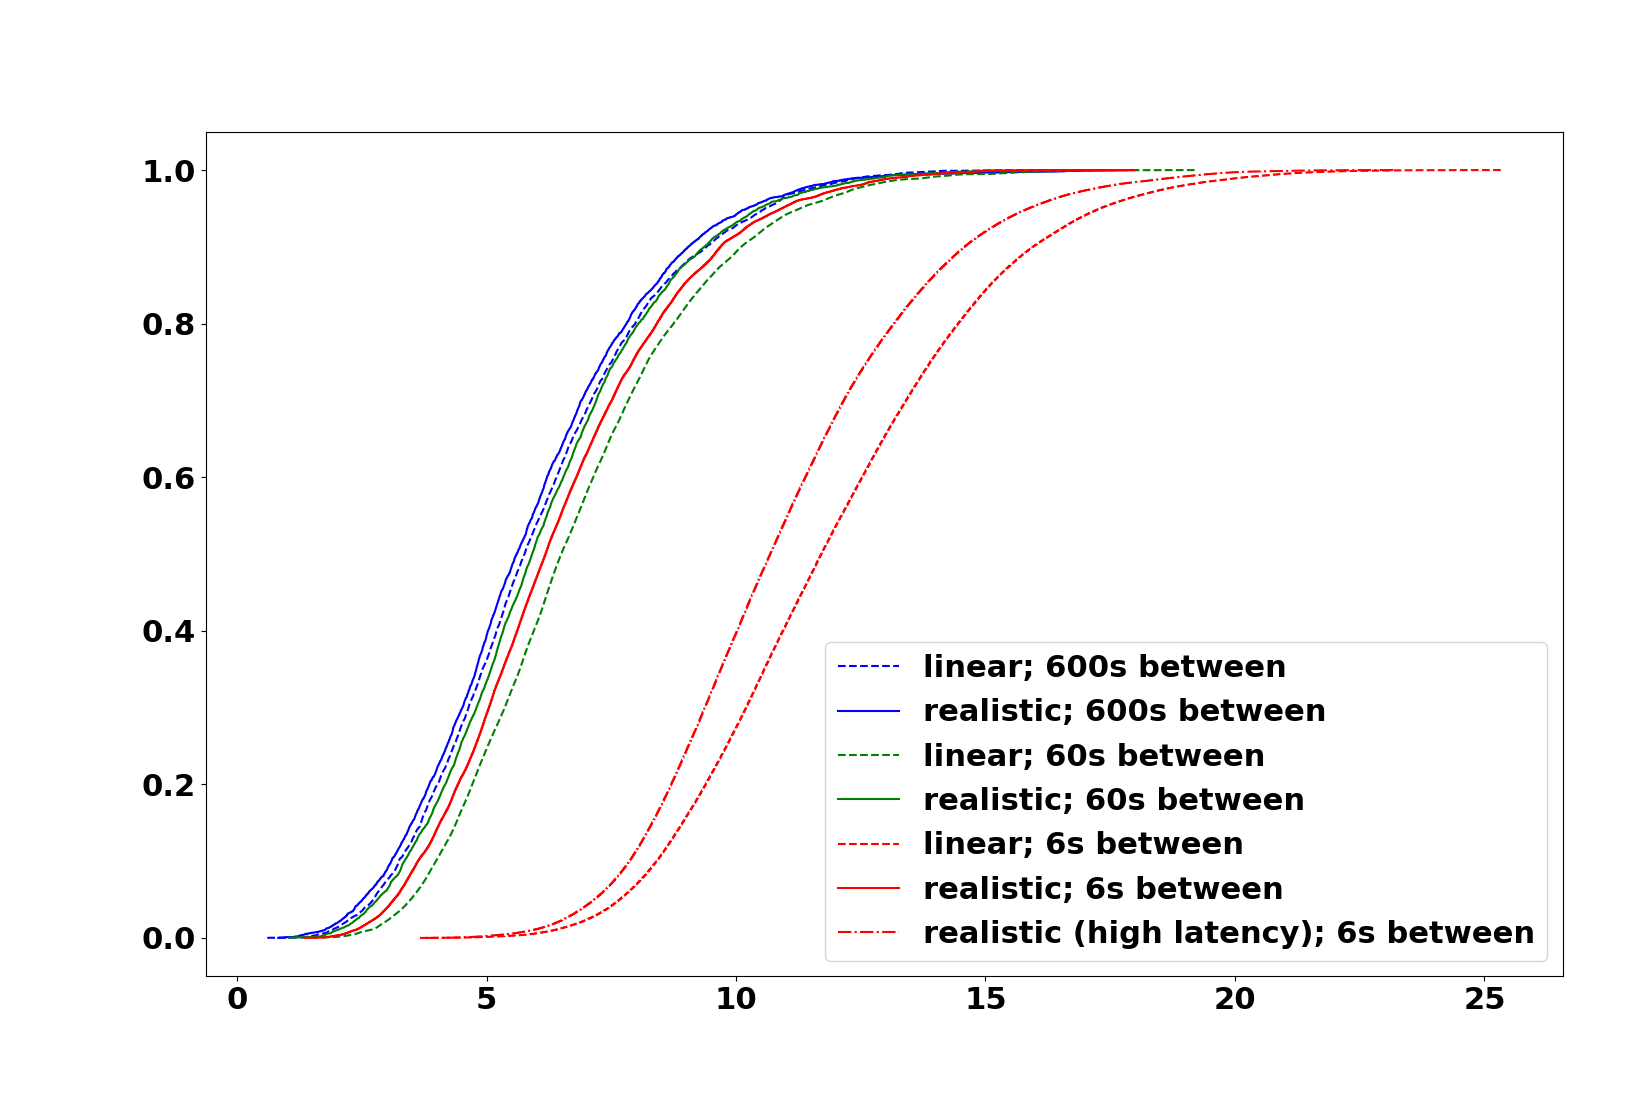
\includegraphics[scale=0.2]{bccomp}

(Note that these results are normalized, meaning that the number of time steps it took each transaction to be in consensus was divided by the generation rate. Otherwise, the higher rate settings give much faster results.) Notice how close the lines are together for 600s and even 60s. This is why we didn't include high latency results for either of those generation rates; the just cluttered that same band. These results are actually less dramatic than we expected.

\subsubsection{Realistic Iota}
\begin{verbatim}
{
    "threadWorkers": 8,
    "numberOfExecutions": 120,
    "topologySelection": "GENERATE_ONCE", 
    "terminationCondition": "NUMBER_OF_GENERATED_TRANSACTIONS",
    "terminationValue": 30,
    "minerPower": {
        "type": "CONSTANT",
        "value": 1
    },

    "topology": {
        "type": "GEOMETRIC_UNIFORM_DELAY",
        "radius": 0.125,
        "numberOfMiners": 500,
        "networkDelay": {
            "type": "EXPONENTIAL",
            "beta": 5
        }
    },
    "protocol": {
        "type": "IOTA",
        "targetTicksBetweenGeneration": 10
    }
}
\end{verbatim}

These parameters reflect the most realistic reflection of Iota that we could find. 500 miners may be a low estimate for the number of miners, but it is not off by an order of magnitude. The topology is an estimate of Iota density, and in reality the density could be sparser. 10 transactions per second is a realistic estimate of generation rate, although a few sources said 100/s. The oft-cited goal of iota is 1000 transactions per second. Network delay is similar to Bitcoin, but is an exponential distribution between 10 and 100 time steps. Again, given that real-world Internet delay is exponential between 100ms and 1000ms, this means that a time step is approximately 100ms. 10 time steps between generation is one transaction every 0.1s or 10 transactions per second.

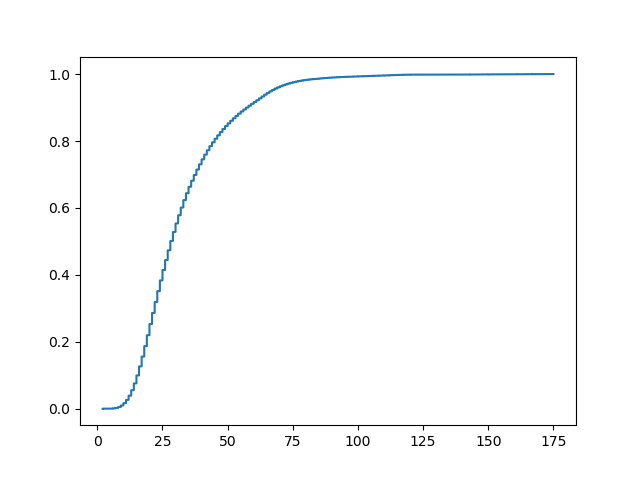
\includegraphics[scale=0.5]{realiotatimes}

Time to consensus is much faster; 3 seconds on average.

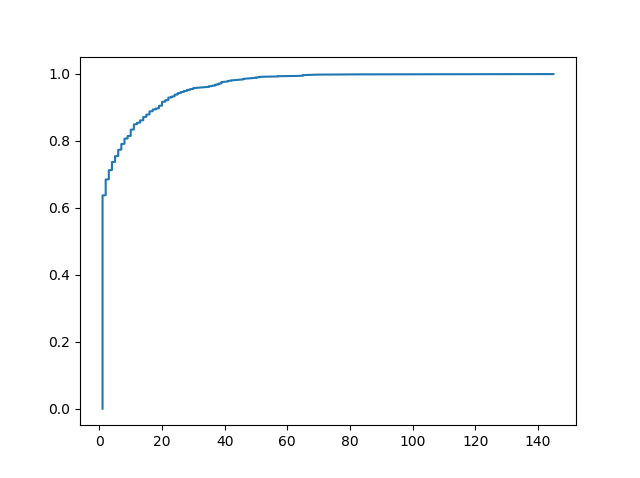
\includegraphics[scale=0.5]{realiotadisc}

Transactions move in and out of consensus, meaning that the protocol is unstable. Instability is observed at all realistic Iota scenarios, but if the parameters are increased to something similar to Bitcoin (more dense, much slower transaction generation rate), then the Tangle starts to become linear (note that the Iota specification \textit{does allow} for transactions to have only one back pointer if there is only one frontier note, or ``tip'', even though all of the previous results use a random second pointer if there is only one) and instability can disappear.

Here, we report transactions that moved out of consensus by a CDF of how long they were out of consensus. The simulation also reports a percentage of transactions that were ever ``disconsensed'' (moved out of consensus after being in it). For these realistic parameters, we see more than 20\% of transactions were ever disconsensed.

\subsubsection{Iota with One Backpointer Vs. Random Backpointer}
Having Iota miners select another random backpointer when there is only one frontier transaction yields different results then when transactions are allowed to have only one backpointer. (Note: I found definite Iota sources that referred to the protocol allowing one backpointer and none that talked about selecting a random second one).

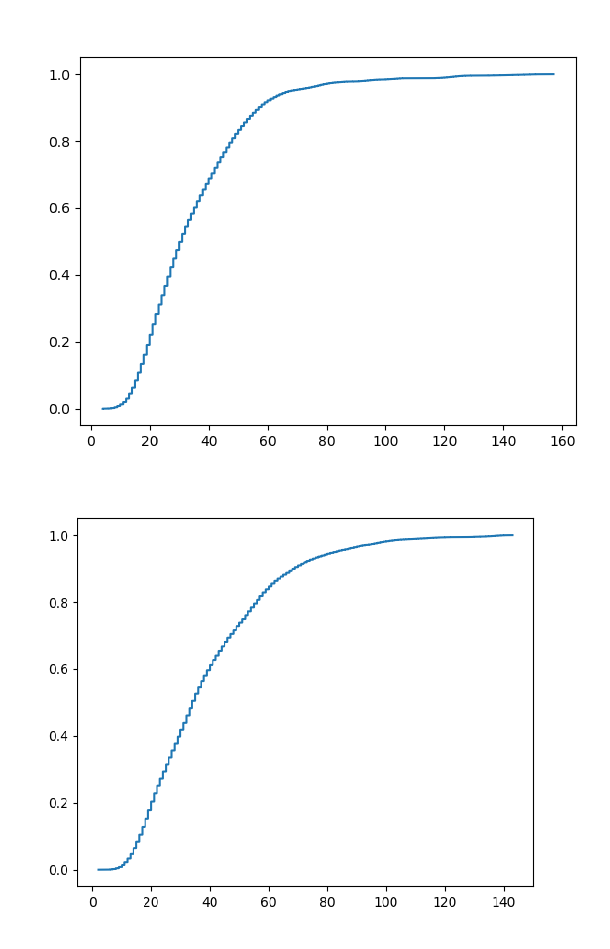
\includegraphics[scale=0.5]{iotaonebackvsrandom}

Top is one backpointer allowed, bottom is required random second pointer. The difference is not extreme. Note that this is very rough as this is only 1 run of the simulation each.

\subsubsection{Digging Deeper into Iota Age Threshold ``Fix'' for Stability}
Not a done deal

Maybe just pushes instability later

Not sure why those initial "worst case" graphs saw it disappearing; a better (direct from json) graph showed plenty of instability still, just later. Note that I didn't choose graph timelines so it's not like I was "only looking from 0-30" explicitly.

Worried that the threshold prevents miners from doing \textit{anything} with a transaction for 30 ticks. Instead tried a fix where if a miner had issued a transaction they couldn't issue another one until it was "age threshold" old. I think that might have looked promising (or at least better).

Take a second to think this through. Should the bare 30 tick wait time work or not??? If yes, why didn't it work?


%out_12_iota_500_miners_10_ticks_exp_5_250_tx_oneback_wait_0
%out_12_iota_500_miners_10_ticks_exp_5_250_tx_oneback_wait_150_fixattempt
%out_12_iota_500_miners_10_ticks_exp_5_250_tx_oneback_wait_30
%out_12_iota_500_miners_10_ticks_exp_5_250_tx_oneback_wait_30_fixattempt
%out_1_iota_500_miners_10_ticks_exp_5_250_tx_oneback_wait_0
%out_1_iota_500_miners_10_ticks_exp_5_250_tx_oneback_wait_30
%out_30_iota_500_miners_10_ticks_exp_5_150_tx_oneback_reiss_wait_0
%out_30_iota_500_miners_10_ticks_exp_5_150_tx_oneback_reiss_wait_30
%out_5_iota_500_miners_10_ticks_exp_5_500_tx_oneback





\end{document}
